% Archivo generado automáticamente con los problemas
\section*{Problems}
Sección: 13_Quantum_electrodynamics
Páginas: 267-269
Contenido:
13.1 Of the tree-level processes in QED, Møller scattering (e−e−→e−e−) is especially
interesting because it involves identical particles.
(a) Calculate the spin-averaged differential cross section for Møller scattering,
e−e−→e−e−. Express your answer in terms of s, t, u and me.
(b) Show that in the non-relativistic limit you get what we guessed by spin-
conservation arguments in Problem 7.3:
dσ
dΩ = m4
eα2
E2
CMp4
1 + 3 cos2θ
sin4θ
,
p2 =
ECM
2
2
−m2
e.
(13.162)
(c) Simplify the Møller scattering formula in the ultra-relativistic limit (me →0).
[Hint: you should get something proportional to (3 + cos2θ)2.]

13.2 Derive Eq. (13.103). It may be helpful to use the formula for scattering in the target
rest frame derived in Problem 5.1.

13.3 Particle decays. Recall that the decay rate is given by the general formula
dΓ =
1
2E1
|M|2 d3p2
(2π)3
1
2E2
· · · d3pn
(2π)3
1
2En
(2π)4δ4(p1 −p2 −· · · −pn). (13.163)
(a) Evaluate the phase-space integrals for 1 →2 decays. Show that the total rate is
Γ(φ →e+ + e−) =
√
1 −4x2
8πmφ
|M|2,
x = me
mφ
.
(13.164)
(b) Evaluate Γ for a particle φ of mass mφ decaying to e+e−of mass me if
1. φ is a scalar, with interaction gSφ ¯ψψ;
2. φ is a pseudoscalar, with interaction igP φ ¯ψγ5ψ;
3. φ is a vector, with interaction gV φμ ¯ψγμψ;
4. φ is an axial vector, with interaction igAφμ ¯ψγμγ5ψ.
(c) Breaking news! A collider experiment reports evidence of a new particle that
decays only to leptons (τ, μ and e) whose mass is around 4 GeV. About 25% of
the time it decays to τ +τ −. What spin and parity might this particle have?

13.4 Show that you always get a factor of −1 in the Feynman rules for each fermionic
loop.

13.5 Consider the following diagram for e+e−→μ+μ−in QED:
(a) How many diagrams contribute at the same order in perturbation theory?
Problems
249
−1.0
−0.5
0.0
0.5
1.0
0
100
200
300
400
500
600
cos θ
Events
−1.0
−0.5
0.0
0.5
1.0
0
100
200
300
400
500
600
cos θ
Events
e+ e− → μ+ μ−
e+ e− → νμνμ
−
Angular distributions in e+e−annihilation produced with a Monte-Carlo simulation.
t
Fig. 13.2
(b) What is the minimal set of diagrams you need to add to this one for the sum to
be gauge invariant (independent of ξ)?
(c) Show explicitly that the sum of diagrams in part (b) is gauge invariant.

13.6 Parity violation. We calculated that e+e−→μ+μ−has a 1 + cos2θ angular depen-
dence (see Eq. (13.78)), where θ is the angle between the e−and μ−directions.
This agrees with experiment, as the simulated data on the left side of Figure 13.2
show. The angular distribution for scattering into muon neutrinos, e+e−→νμ¯νμ, is
very different, as shown on the right side of Figure 13.2, where now θ is the angle
between the e−and νμ directions.
(a) At low energy, the total cross section, σtot, for e+e−→νμ¯νμ scattering grows
with energy, in contrast to the total e+e−→μ+μ−cross section. Show that this
is consistent with neutrino scattering being mediated by a massive vector boson,
the Z. Deduce how σtot should depend on ECM for the two processes.
(b) Place the neutrino in a Dirac spinor ψν. There are two possible cou-
plings we could write down for the ν to the new massive gauge boson:
gV ¯ψν /Zψν + gA ¯ψν /Zγ5ψν. These are called vector and axial-vector couplings,
respectively. Assume the Z couples to the electron in the same way as it cou-
ples to neutrinos. Calculate the full angular dependence for e+e−→νμ¯νμ as a
function of gV and gA (you can drop masses).
(c) What values of gV and gA reproduce Figure 13.2? Show that this choice is equiv-
alent to the Z boson having chiral couplings: it only interacts with left-handed
fields. Argue that this is evidence of parity violation, where the parity operator
P is reflection in a mirror: ⃗x →−⃗x.
(d) An easier way to see parity violation is in β-decay. This is mediated by charged
gauge bosons, the W ±, that are “unified” with the Z. Assuming they have the
same chiral couplings as the Z, draw a diagram to show that the electron coming
out of C60 →Ni59 +e−+ ¯ν will always be left-handed, independent of the spin
of the cobalt nucleus. What handedness would the positron be in anti-cobalt
decay: C
60 →Ni
59 + e+ + ν?
(e) If you are talking to aliens on the telephone (i.e. with light only), tell them how
to use nuclear β-decay to tell clockwise from counterclockwise. For this, you
will need to figure out how to relate the L in ψL to “left” in the real world.
250
Quantum electrodynamics
You are allowed to assume that all the materials on Earth are available to them,
including things such as cobalt, and lasers.
(f) If you meet those aliens, and put out your right hand to greet them, but they put
out their left hand, why should you not shake? (This scenario is due to Feynman.)
(g) Now forget about neutrinos. Could you have the aliens distinguish right from left
by actually sending them circularly polarized light, for example using polarized
radio waves for your intergalactic telephone?

13.7 One should be very careful with polarization sums and in giving physical inter-
pretations to individual Feynman diagrams. This problem illustrates some of the
dangers.
(a) We saw that the t-channel diagram for Compton scattering scales as Mt ∼
1
t . Calculate |Mt|2 summed over spins and polarizations. Be sure to sum over
physical transverse polarizations only.
(b) Calculate |Mt|2 summed over spins and polarizations, but do the sum by replac-
ing ϵμϵ⋆
ν by −gμν. Show that you get a different answer from part (a). Why is
the answer different?
(c) Show that when you sum over all the diagrams you get the same answer whether
you sum over physical polarizations or use the ϵμϵ⋆
ν →−gμν replacement. Why
is the answer the same?
(d) Repeat this exercise for scalar QED.

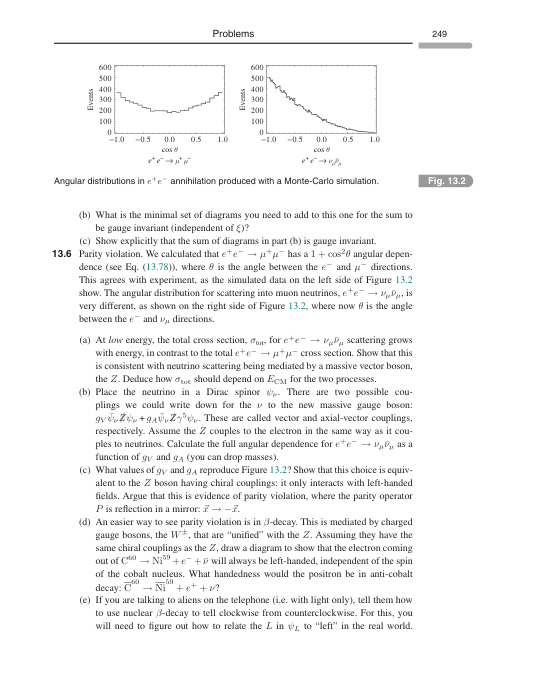
\includegraphics{./figs/13_Quantum_electrodynamics_page_269.png}

---

